\documentclass[11pt]{article}
\usepackage{geometry}                % See geometry.pdf to learn the layout options. There are lots.
\geometry{letterpaper}                   % ... or a4paper or a5paper or ... 
%\geometry{landscape}                % Activate for for rotated page geometry
%\usepackage[parfill]{parskip}    % Activate to begin paragraphs with an empty line rather than an indent
\usepackage{graphicx}
\usepackage{caption}
\usepackage{amssymb}
\usepackage{wrapfig}
\usepackage{amsmath}
\usepackage{epstopdf}
\DeclareGraphicsRule{.tif}{png}{.png}{`convert #1 `dirname #1`/`basename #1 .tif`.png}

\title{Playing with the E\&M Toy Model:\\A Charged Spinning Sphere}
\date{}                                           % Activate to display a given date or no date

\begin{document}
\maketitle
\section{Comparing the E\&M Analogy with Kerr}
I argued in [insert section number here] that E\&M is a strong analog to gravity.  That was a generic field theoretic argument; let's take advantage of this to get some concrete predictions.  Taking the analogy as valid, then, we can construct a toy model to compare with Kerr.

To review, mapping gravity to electromagnetism, we can say:

\begin{align}
m &\rightarrow q   \text{ (mass becomes charge)}\\
G &\rightarrow \frac{1}{4\pi\epsilon_0} \text{ (constants switch)}\\
+ &\rightarrow - \text{ (gravity is attractive; electricity, repulsive)}
\end{align}

Then, making special relativistic considerations, we can derive necessary magnetic fields as corrections to both electricity and gravity.
\begin{figure}[h]
  \begin{center}
    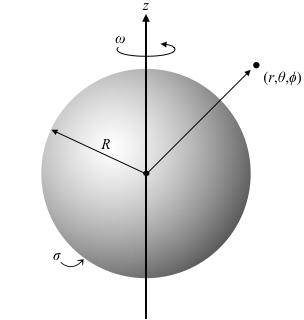
\includegraphics[scale=.65]{/Users/alexdeich/thesis/latex/figs/charged_spinning_sphere.png}
  \end{center}
  \caption{}
  \label{fig:charged_spinning_sphere}
\end{figure}

So, we're studying orbits in the Kerr spacetime, which is the consequence of a spinning mass.  Accounting for the above mapping then, we should expect the analogous E\&M system to be represented by Fig.\ref{fig:charged_spinning_sphere}:  A charged spinning sphere.  Specifically, we want to study the orbit of a charged particle near the sphere.  Finally, to the point of this thesis, we seek how the orbits of the particles change when the spin of the central sphere changes.

\section{A Description of the Relevant Magnetic Vector Potential}
All quantities refer to Fig.\ref{fig:charged_spinning_sphere}.  Our system is a solid sphere of radius $R$ with constant surface charge density $\sigma$, rotating about the $z$ axis with some angular frequency $\omega$.

 The magnetic vector potential at an arbitrary point $(r,\theta,\phi)$ outside the sphere is given by $\mathbf{A} = \frac{\mu_0R^4\sigma}{3}\frac{\sin\theta}{r^2}\mathbf{\hat{\phi}}$.  The derivation for this is reproduced in Appendix [insert number].  For our purposes, it is helpful to reparameterize the vector potential with the angular momentum, $l$ and total charge $Q$ instead\footnote{This change is made using the angular momentum per unit mass, $I\omega/M$, with the moment of inertia of a sphere, $I = 2MR^2/5$.}:
 \begin{equation}
 \mathbf{A} = \frac{1}{2}\frac{\mu_0 Q l}{4\pi}\frac{\sin\theta}{r^2}\mathbf{\hat{\phi}}
 \end{equation}
The electric potential is unchanged from a static sphere: $V = \frac{Q}{4\pi\epsilon_0r}$.


Then, to probe the trajectories of a particle of charge $q$ near the spinning sphere, we need to look at the Lagrangian

\begin{equation}\label{eq:particle_lagr}
L = \frac{1}{2}m\left(\dot{r}^2 + r\cos\dot{\theta} + r\sin^2\theta\dot{\phi}\right) - \frac{qQ}{4\pi\epsilon_0r} + \frac{mu_0qQl}{8\pi}\frac{sin^2\theta}{r}\dot{\theta}.
\end{equation}
 
 






\end{document}  